\section{Shared Memory}
\label{sec:omp}

\todorev{Last revised on Sat, June 30 at 22:15 by pfac}

A shared memory parallel version of \polu was implemented using the OpenMP interface. The main feature about this API is that the program itself remains almost equal to the sequential version, requiring only the addition of the necessary directives and the adaptation of the code to remove dependencies.

Both core functions were parallelized just by adding a \texttt{parallel for} directive to the internal loops. The number of threads issued in each parallel zone is given as the second argument of the program, and defaults to the maximum number of threads supported by the hardware in the absence of the argument.

	\subsection{Load Balance}
% \todo[inline]{Describe the static scheduling with OpenMP and explain that all the iterations make the same operations in every function}

Both core functions are mostly homogeneous in its parallel implementation. In \computeflux, the two branches perform the same amount of operations whether they are followed or not. In \update, the heaviest part of the workload is constant (products and divisions), and it only differs in the number of edges contributing to the edge. While this value may cause the function to become heterogeneous, this is highly dependent on the mesh used (the test case used in \cref{sec:700} has 3 edges in every cell).

By default, the OpenMP interface uses static scheduling, where iterations are assigned to threads in a \textit{round-robin} pattern. Since the number of edges and cells is a constant throughout the entire execution, this guarantees the best load balancing among threads.

\subsection{Limitations}
% \todo[inline]{Describe the locality problems}
% \todo[inline]{Opportunity to show here that cute image that displays locality of the mesh}

The main problem with this implemetation is data locality. While these issues are softened using a SOA approach, and the method is a first order one, the algorithm is still not very cache friendly in either of the core functions.

In \computeflux, each edge requires access to data from the two adjacent cells. While the access to edges is contiguous, access to cells is not for most of the iterations. Yet, border edges do not require the second edge.

\update on the other hand requires access to all the edges in a cell, which are always more than two. Analogously, the access to cells is contiguous, but the access to edges is not. Since each edge has more edges, than an edge has adjacent cells, and since no edge may be neglect for any cell, this function is most likely the bottleneck of the main loop.
 \subsection{Results}

\Cref{fig:results:omp} shows the speedups obtained with the two optimized sequential versions parallelized using OpenMP, for different numbers of threads.

It is clear to see that the \soa version obtained the best results. Even considering the speedup obtained compared to the sequential \aos version, this approach to the structures implementation scales better, allowing to take further advantage of the hardware resources.

The best results were obtained using 12 threads, which in SeARCH Group Hex nodes represents the full hardware support, disregarding \intel Hyperthreading technology. While this allows two threads to run in the same processor core, it rarely is benefitial for the program execution.

\begin{figure}[!htp]
	\centering
	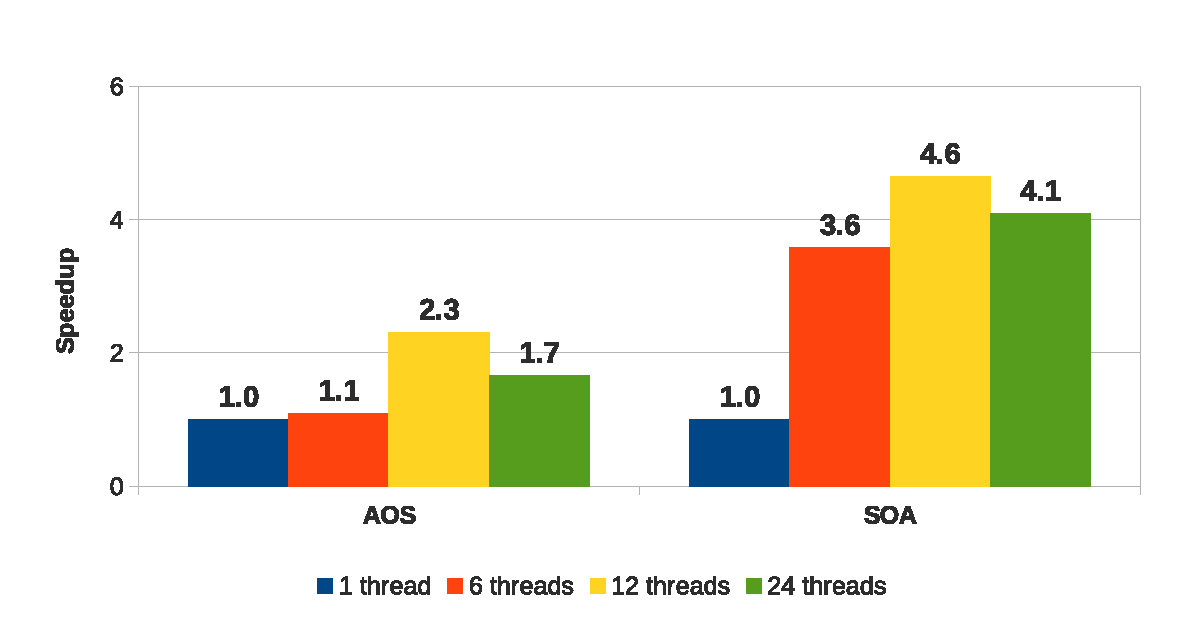
\includegraphics[width=\columnwidth]{images/graph_comparison_omp.eps}
	\caption{Speedup results for the two optimized sequential versions, parallelized with OpenMP. Original implementation used as reference.}
	\label{fig:results:omp}
\end{figure}
